\title{LeapYear Algorithm}
\author{
        Tue Edmund Gyhrs
        \\tugy@itu.dk
}
\date{\today}

\documentclass[12pt]{article}
\usepackage{graphicx}
\graphicspath{ {./LaTeX/images/} }
\begin{document}
\maketitle
\begin{figure}[h]
    \centering
    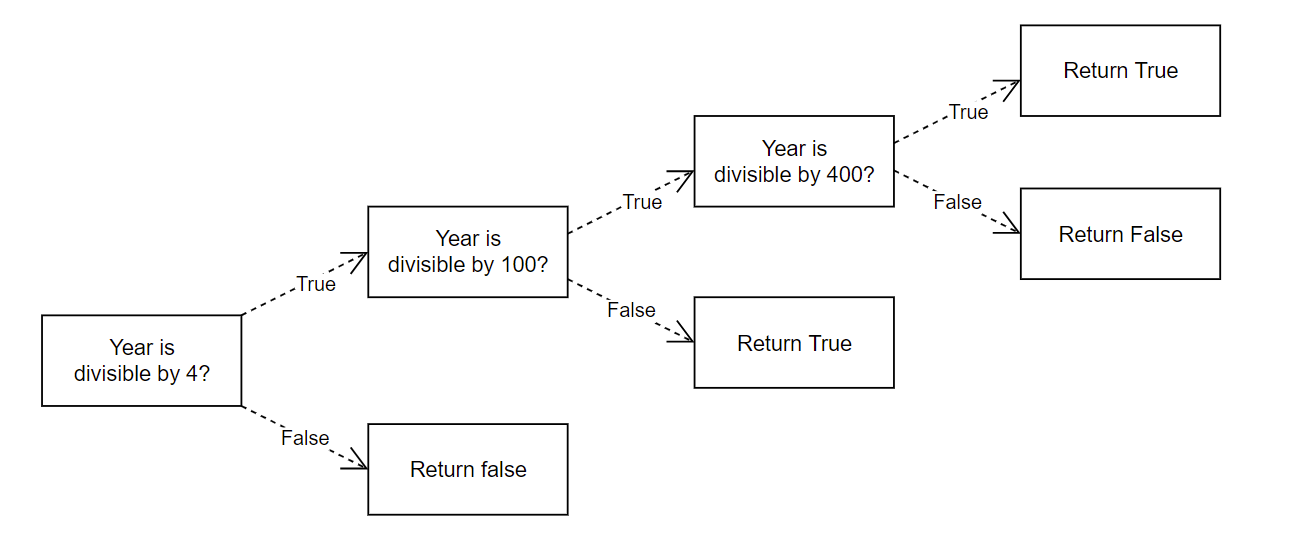
\includegraphics[width=0.8\textwidth]{LaTeX/images/AlgorithmForLeapYear.PNG}
    \caption{isLeapYear algorithm}
\end{figure}
The algorithm first checks to see if the year is divisible by 4. False means the year was not a leap year and true means we check if it is divisible by 100. False here means it can't ever be divisible by 400 so it is a leap year aswell. True leads us to the final question, "is the year divisible by 400?". True means yes it is and false means no it isn't.
\end{document}